\usetikzlibrary{arrows.meta,positioning}
\chapter{Methodology}
\label{chap:methodology}
At each local midnight, the forecaster estimates the next 24 hourly energy values at a target charging location. With only a short history at that location, the model can start from weights learned at other locations in the same dataset and city. We examine two subsequent decisions. During training, how strongly should the target encoder be constrained to preserve the source representation? At forecast time, how much weight should each of two adaptation trajectories receive?

\section{Forecasting workflow}
We train the source model on eligible historical windows from source identifiers. Each dataset--city group and random seed has its own checkpoint. In the historical study, seven groups and three seeds yield 21 source checkpoints. For each target identifier, history budget and seed, adaptation starts separately from the corresponding checkpoint. With no complete examples in the target prefix, initial adaptation performs zero optimizer steps.

Figure~\ref{fig:ch4fusion} follows one forecast from the pretrained forecaster through two target models. Both models use the same target history and future calendar. Once the actual demand arrives, the stored forecasts supply the errors for the next weight update. Section~\ref{sec:retention} describes the earlier experiment that deploys a single branch at a time.

\begin{figure}[htbp]\centering
\resizebox{\linewidth}{!}{\definecolor{evBlue}{HTML}{205B82}
\definecolor{evRust}{HTML}{A74731}
\begingroup\def\baselinestretch{1}
\begin{tikzpicture}[x=1cm,y=1.55cm,>=Latex,
 box/.style={draw=evBlue!65,fill=evBlue!4,rounded corners=2pt,text width=4.10cm,align=center,inner sep=5pt,minimum height=1.18cm,font=\small},
 warm/.style={box,draw=evRust!65,fill=evRust!4},
 pathline/.style={->,draw=black!70,line width=.65pt},
 lab/.style={font=\scriptsize,fill=white,inner sep=2pt}]
\node[box] (src) at (0,3.9) {\textbf{Source training}\\Established sites\\GRU encoder and forecast head};
\node[box] (init) at (5.3,3.9) {\textbf{Target adaptation}\\Source initialization\\(7, 14 or 28 days initially)};
\draw[pathline] (src)--(init);
\node[box] (input) at (10.6,3.9) {\textbf{Each forecast origin}\\Previous 24 hours ($24\times7$)\\Next-day calendar ($24\times5$)};
\node[box] (st) at (2.65,1.50) {\textbf{Stable GRU}\\$F+R$, frozen source reference\\Train on the newly arrived day};
\node[warm] (fa) at (7.95,1.50) {\textbf{Fast GRU}\\$F$, no retention penalty\\Train on up to seven recent days};
\coordinate (shared) at (5.3,2.65);
\draw[draw=black!70,line width=.65pt] (init.south)--(shared);
\draw[draw=black!70,line width=.65pt] (input.south) |- (shared);
\fill[black!70] (shared) circle (1.3pt);
\draw[pathline] (shared)--++(0,-.22) -| (st.north);
\draw[pathline] (shared)--++(0,-.22) -| (fa.north);
\node[box] (mix) at (5.3,-.70) {\textbf{Issue 24 hourly estimates}\\$\hat y_t=w_t\hat y_{S,t}+(1-w_t)\hat y_{F,t}$};
\draw[pathline] (st.south) |- ([yshift=2pt]mix.west);
\draw[pathline] (fa.south) |- ([yshift=2pt]mix.east);
\node[box] (score) at (5.3,-2.65) {\textbf{Score the saved expert forecasts}\\24 labels arrive\\Compute normalized daily MAE};
\draw[pathline] (mix)--(score);
\node[warm] (next) at (10.6,-2.65) {\textbf{Next forecast weight}\\Update with expert losses\\$w^+=0.1+0.8p$};
\draw[pathline] (score)--(next);
\draw[pathline,draw=evRust] (next.north) |- ([yshift=-4pt]mix.east);
\end{tikzpicture}\endgroup
}
\caption{Source initialization, target adaptation and forecast fusion.}\label{fig:ch4fusion}
\end{figure}

\section{GRU encoder and training objective}
The input window contains 24 hourly vectors with seven features each. The prediction head also receives five known calendar features for each future hour. A standard gated recurrent unit (GRU) encodes the history \cite{cho2014}. The encoder has two layers of width 64, zero dropout and a fresh hidden state for each window.

The last-layer final state $h_{24}\in\mathbb R^{64}$ is concatenated with the 120 flattened future-calendar values. The head applies a width-64 linear layer, ReLU, a 24-output linear layer and Softplus. The primary forecaster has 52,376 trainable parameters.


Figure~\ref{fig:gru-forward} follows the two inputs through a single forecaster. The calendar enters after the history has been encoded. During target training, the same 64-dimensional history representation also enters the retention penalty.
\begin{figure}[htbp]\centering
\resizebox{.95\linewidth}{!}{\begingroup\def\baselinestretch{1}
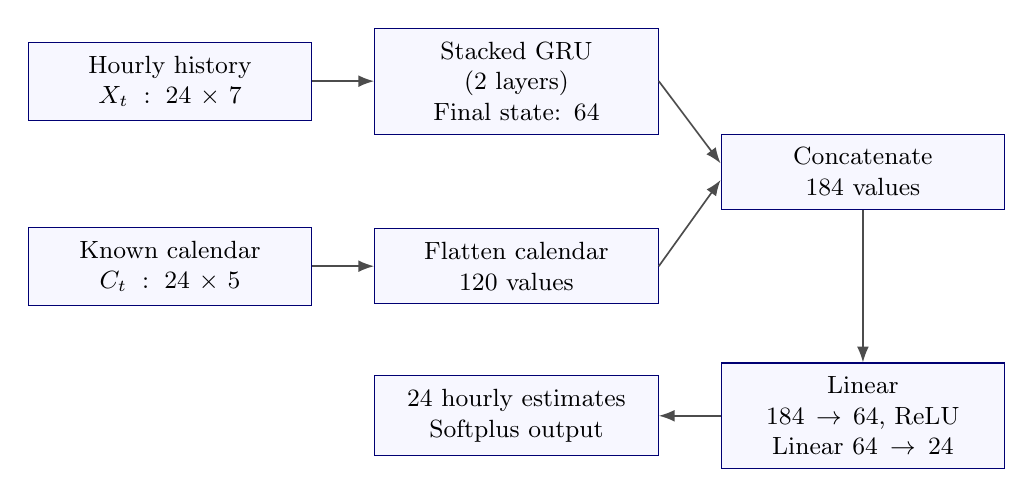
\begin{tikzpicture}[x=1cm,y=1cm,>=Latex,
 box/.style={draw=blue!45!black,fill=blue!3,align=center,text width=3.25cm,inner sep=5pt,font=\small},
 a/.style={->,semithick,draw=black!70}]
\node[box] (x) at (0,0) {Hourly history\\$X_t:24\times7$};
\node[box] (c) at (0,-2.35) {Known calendar\\$C_t:24\times5$};
\node[box] (h) at (4.4,0) {Stacked GRU (2 layers)\\Final state: 64};
\node[box] (f) at (4.4,-2.35) {Flatten calendar\\120 values};
\node[box] (cat) at (8.8,-1.15) {Concatenate\\184 values};
\node[box] (out) at (4.4,-4.25) {24 hourly estimates\\Softplus output};
\node[box] (head) at (8.8,-4.25) {Linear $184\to64$, ReLU\\Linear $64\to24$};
\draw[a](x)--(h);\draw[a](c)--(f);\draw[a](h.east)--([yshift=3pt]cat.west);
\draw[a](f.east)--([yshift=-3pt]cat.west);
\draw[a](cat.south)--(head.north);
\draw[a](head)--(out);
\end{tikzpicture}\endgroup
}
\caption{History encoder and calendar-conditioned forecast head.}\label{fig:gru-forward}
\end{figure}

\subsection{Forecast loss and latent retention}

Li et al.~\cite{li2018} use pretrained parameters as the reference for an explicit transfer penalty. Here we use the frozen source encoder as a reference in representation space and scale each coordinate by its source variability. The target GRU minimizes a forecast error $F_B$ and a latent penalty $R_B$ over a batch $B$ of complete days. For example $j$ and forecast hour $q$, $\widetilde y$ and $\widehat{\widetilde y}$ denote observed and predicted energy normalized by the target scale.
\begin{equation}\begin{aligned}
L_B(\theta,\lambda)&=F_B(\theta)+\lambda R_B(\theta),\\
F_B(\theta)&=\frac{1}{24|B|}\sum_{j\in B}\sum_{q=1}^{24}
|\widehat{\widetilde y}_{j,q}(\theta)-\widetilde y_{j,q}|,\\
R_B(\theta)&=\frac{1}{64|B|}\sum_{j\in B}\sum_{k=1}^{64}
\left(\frac{h_k(x_j;\theta)-h_k(x_j;\theta_s)}{s_k+0.001}\right)^2 .
\end{aligned}\label{eq:total}\end{equation}
In Equation~\eqref{eq:total}, both encoders process the same target history $x_j$. The source parameters $\theta_s$ and population standard deviation (computed over source training encodings) $s_k$ of each latent coordinate stay fixed. Adam updates the target parameters $\theta$. A positive $\lambda$ penalizes divergence from the source encoding. At $\lambda=0$, the target learns from forecast error alone and retains its source initialization.

\section{Fixed retention and coefficient calibration}
Historical fixed retention uses a constant $\lambda=1$. The original selector considers $\{0,0.1,1\}$ and starts from a common target adaptation at $\lambda=0.1$. These coefficients define the historical comparison. Their effective penalty strength depends on the gradients measured during target training.

The twelve-entity Development study uses independent trajectories at the same three coefficients but selects its Fixed comparator on the four calibration entities. It selects $\lambda=1,1,0$ for 7-, 14- and 28-day prefixes. Thus its Fixed row is not identical to the historical fixed-one recipe. A zero coefficient in that row still retains Source initialization.

\subsection{Expanded fixed-coefficient diagnostic}
The four-target coefficient study evaluates 21 real coefficients, including zero, using a finite Gaussian-process/expected-improvement search on positive log coefficients plus a coverage sensitivity grid. Acquisition is maximized approximately on 4,097 numeric grid points. Calibration averages forecast MAE equally across entities and paired seeds on the first 28 scheduled origins:
\begin{equation}
\lambda^*=\underset{\lambda\in\Lambda_{\rm measured}}{\operatorname{argmin}}\;
\frac{1}{4}\sum_{i=1}^4\frac{1}{3}\sum_{s=42}^{44}
\operatorname{MAE}^{\rm Cal}_{i,s}(\lambda).
\label{eq:fixedselection}
\end{equation}
The positive search interval is derived from prefix-only gradient-balance coefficients after three unregularized target epochs: its lower endpoint is 0.01 times the minimum measured balance coefficient, and its upper endpoint is 100 times the maximum. These factors deliberately span weak to dominant local penalty gradients; they are engineering coverage choices. Zero is evaluated separately. The resulting positive search interval was $[0.00038785,33.84425]$. The best measured coefficient lay inside the interval. Exact ties in calibration MAE favour the smaller coefficient. The search follows the Gaussian-process approach to hyperparameter optimization \cite{snoek2012}.
Equation~\eqref{eq:fixedselection} selected $\lambda^*=0.798445$ among the measured candidates. Chapter~5 reports the measured gradient ratios and forecast errors for representative coefficients.

\section{Adaptive retention mechanisms}\label{sec:retention}
\subsection{Confidence-gated block selection}
\begin{figure}[htbp]
\centering\resizebox{.96\linewidth}{!}{\definecolor{FlowBlue}{HTML}{2166AC}
\definecolor{FlowRed}{HTML}{B2182B}
\begin{tikzpicture}[x=1cm,y=1cm,>=Latex,every node/.style={font=\footnotesize,align=center},
box/.style={draw=black!40,rounded corners=2pt,fill=white,inner sep=6pt,text width=3.5cm,minimum height=1.1cm},
flow/.style={->,draw=black!65,line width=.7pt}]
\node[box,fill=FlowBlue!7,draw=FlowBlue!65] (start) at (0,0) {\textbf{Selected trained state}\\Model and Adam moments};
\node[box,fill=FlowBlue!7,draw=FlowBlue!65] (fork) at (5.2,0) {\textbf{Clone at block start}\\$\lambda\in\{0,0.1,1\}$};
\node[box] (pred) at (10.4,0) {\textbf{Predict and learn}\\Three causal branches};
\node[box] (labels) at (10.4,-2.8) {\textbf{Complete arrived errors}\\Paired within the 14-day block};
\node[box,fill=FlowRed!6,draw=FlowRed!65] (decision) at (5.2,-2.8) {\textbf{Bootstrap lower bounds}\\$n\ge7$ paired days\\Switch only if $L_c>0$};
\node[box,fill=FlowBlue!7,draw=FlowBlue!65] (carry) at (0,-2.8) {\textbf{Carry selected branch}\\Keep its trained model and Adam};
\draw[flow] (start)--(fork);\draw[flow] (fork)--(pred);\draw[flow] (pred)--(labels);
\draw[flow] (labels)--(decision);\draw[flow] (decision)--(carry);\draw[flow] (carry)--(start);
\end{tikzpicture}
}
\caption{Historical confidence-guided retention selection.}\label{fig:retention}
\end{figure}
Figure~\ref{fig:retention} shows the original retention controller. It begins each 14-day block by cloning the selected model and Adam state into three branches, one per retention coefficient. All branches forecast causally and train on the same eligible data. Only the active branch supplies the deployed forecast. At the next boundary, complete arrived daily errors within the block are paired.

We use moving-block resampling for dependent observations \cite{kunsch1989}. Our switching rule compares the errors of challenger $c$ and active branch $a$ on the same completed day $d$. We define
\begin{equation}\begin{aligned}
D_{c,d}&=e_{a,d}-e_{c,d},\\
L_c&=Q_{0.025}\!\left(\overline{D}_{c}^{*(1)},\ldots,
\overline{D}_{c}^{*(2000)}\right).
\end{aligned}\label{eq:lcb}\end{equation}
Positive differences favor the challenger. Resamples concatenate noncircular overlapping segments of three chronological valid daily observations, trimming to the original valid-day count. Both challengers use identical sampled indices. The 0.025 tail implements the specified two-challenger adjustment with interval parameter 0.05. Quantiles are linearly interpolated.

If fewer than seven complete days are available, or no challenger has $L_c>0$, the active branch is retained. Otherwise the controller selects the greatest qualifying lower bound, breaking exact ties by proximity to the current coefficient and then ascending coefficient order. The selected \emph{trained} model and optimizer continue forward, and are cloned again at the new block start. Keeping the active branch does not restore its block-start weights.

Algorithm~\ref{alg:retention} gives the order of forecasting, learning and branch selection. The lower bound describes differences observed in the completed block. Missing days compress the sequence used for resampling.

\begin{algorithm}[htbp]
\caption{Retention selection at a target station}\label{alg:retention}
\begin{algorithmic}[1]
\State Initialize the target from source and adapt on the eligible prefix at $\lambda=0.1$.
\For{each 14-day block}
  \State Copy the active model and Adam state to branches with $\lambda\in\{0,0.1,1\}$.
  \For{each forecast origin in the block}
    \State Update each branch on eligible earlier feedback and save its new forecast.
    \State Issue the forecast from the active branch.
  \EndFor
  \State At the boundary, process eligible arrivals and pair complete daily errors.
  \If{at least seven paired days are available}
    \State Compute challenger bounds using Equation~\eqref{eq:lcb}.
    \State Select the highest positive bound if one exists, using the tie rule above.
  \EndIf
  \State Carry the selected trained model and its Adam state into the next block.
\EndFor
\end{algorithmic}
\end{algorithm}

\subsection{Common-bank online selection}
The separate twelve-entity study trains independent constant-coefficient trajectories instead of reforking a chosen state every block. Its past-MAE selector and confidence selector choose outputs from this same bank, starting from the calibration-selected Fixed trajectory. Both rules nominate the candidate with the lowest past MAE. The confidence variant gates that same nomination before switching. It uses seven-day blocks, at least five complete days, segment length three, 2,000 resamples and the same zero-margin principle.

This matched bank compares two output-selection rules. It is not a rerun of the original 14-day model-reforking procedure. 

A separate four-target study tested a continuous coefficient. It used two earlier days for a virtual training step and a more recent observed day to estimate how changing $\lambda$ would affect forecast error. Appendix~\ref{app:continuous} gives the update and calibration settings. A further calibration experiment tested a shadow model and transferred its proposed coefficient only after sufficient paired evidence.


Figure~\ref{fig:continuous-step} shows one eligible update of the continuous controller. The virtual step changes a temporary copy of the parameters. The validation gradient determines the coefficient used by the real optimizer when the newly arrived example enters training.
\begin{figure}[htbp]\centering
\resizebox{.95\linewidth}{!}{\begingroup\def\baselinestretch{1}
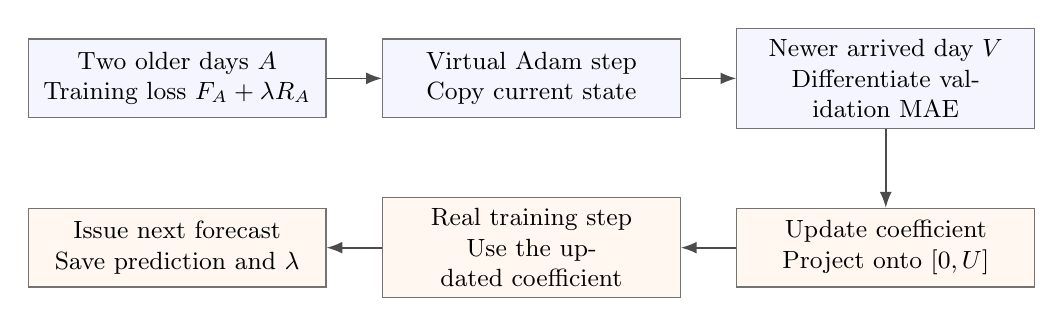
\begin{tikzpicture}[x=1cm,y=1cm,>=Latex,
 box/.style={draw=black!55,align=center,text width=3.5cm,minimum height=1.0cm,inner sep=4pt,font=\small},
 a/.style={->,semithick,draw=black!70}]
\node[box,fill=blue!4] (a) at (0,0) {Two older days $A$\\Training loss $F_A+\lambda R_A$};
\node[box,fill=blue!4] (v) at (4.5,0) {Virtual Adam step\\Copy current state};
\node[box,fill=blue!4] (g) at (9,0) {Newer arrived day $V$\\Differentiate validation MAE};
\node[box,fill=orange!6] (lambda) at (9,-2.15) {Update coefficient\\Project onto $[0,U]$};
\node[box,fill=orange!6] (real) at (4.5,-2.15) {Real training step\\Use the updated coefficient};
\node[box,fill=orange!6] (issue) at (0,-2.15) {Issue next forecast\\Save prediction and $\lambda$};
\draw[a](a)--(v);\draw[a](v)--(g);\draw[a](g)--(lambda);\draw[a](lambda)--(real);\draw[a](real)--(issue);
\end{tikzpicture}\endgroup
}
\caption{Virtual and real updates in the continuous retention experiment.}\label{fig:continuous-step}
\end{figure}

\section{Adaptive fusion of two retention experts}
\subsection{Complementary trajectories}


The fusion extension in Figure~\ref{fig:ch4fusion} retains two GRUs initialized from the source checkpoint at epoch 10. The stable expert is the historical Fixed model: $\lambda_S=1$, three initial target epochs when complete prefix examples exist, learning rate 0.001, and one online epoch on each newly arrived complete daily example. The historical comparison reuses the forecasts previously issued by this model.

The fast expert uses $\lambda_F=0$, the same three initial epochs and learning rate, and one online epoch over available complete examples in the seven calendar days ending at the arrived example's forecast origin. The window may include permitted prefix examples, contains at most seven complete daily examples, and fits one optimizer step. It never includes labels that have not arrived.

The experts differ in both retention and update memory. A gain from combining them therefore cannot be attributed solely to different coefficients. Both start from Source; the fast expert is not target-only. Their coefficients remain constant throughout fusion.

\subsection{Weight update}
For stable weight $w_t$, the issued 24-hour forecast is
\begin{equation}
\hat y_{t,q}=w_t\hat y_{S,t,q}+(1-w_t)\hat y_{F,t,q}.
\label{eq:fusion}\end{equation}
Once all 24 labels for an earlier day $d$ arrive, each expert's loss $\ell_{e,d}$ is its mean absolute hourly error in kWh divided by the target energy scale $c_i$. Both losses use the forecasts stored at issue time.
At feedback event $k$, we apply the two-expert Fixed-share update of Herbster and Warmuth \cite{herbster1998} to the normalized daily losses. The resulting weight applies to subsequent forecasts.
\begin{equation}\begin{aligned}
p_k&=\frac{w_k\exp(-\eta\ell_{S,d})}
{w_k\exp(-\eta\ell_{S,d})+(1-w_k)\exp(-\eta\ell_{F,d})},\\
w_{k+1}&=(1-\alpha)p_k+\alpha(1-p_k)\\
&=\alpha+(1-2\alpha)p_k.
\end{aligned}\label{eq:fixedshare}\end{equation}
The implementation uses equivalent log-odds arithmetic. Calibration selects $w_0=0.430782$, $\eta=0.1$ and $\alpha=0.1$. Updated weights consequently lie in $[0.1,0.9]$. This bound follows from sharing, not from a lambda search. No complete feedback means no weight update; elapsed time alone does not decay the weight.

The weight at forecast origin $t$ is the state after all eligible feedback events $k$ preceding issuance have been processed. The runner applies Equation~\eqref{eq:fixedshare} to earlier feedback before issuing the current forecast with Equation~\eqref{eq:fusion}. Both experts continue training under their respective fixed retention coefficients.

\subsection{Calibration and matched fusion controls}
Four calibration entities and seeds 42--44 compare fast windows of 3, 7 and 14 days with learning rates 0.001 and 0.003. For each pair, a static stable weight minimizes equal-cell Calibration MAE on $[0,1]$ via the weighted-median solution of the convex absolute-error objective. This selects the seven-day, 0.001 recipe and the initial weight above.

Nine weight-controller candidates cross $\eta\in\{0.1,1,10\}$ and $\alpha\in\{0.001,0.01,0.1\}$. Calibration selects the final settings before their historical full-scope comparison. The same recipe is carried to all namespaces and histories without per-namespace recalibration. These bounded engineering grids do not establish global optimality.

The decisive control is static fusion with the same stable and fast forecasts and fixed $w_0$. Fast-only tests one component. Equal 50/50 fusion and loss-free sharing are posthoc diagnostics; in loss-free sharing, the posterior equals the prior before the same share step. This retains attraction toward one-half while removing the expert-loss signal.

\section{Training setup and evaluation}
\subsection{Implementation and hyperparameters}
The 46-target Development evaluation ran in Python 3.12.13 with PyTorch 2.11.0. Table~\ref{tab:ch4training} gives its locked training settings. Each seed identifies the source checkpoint and pairs the methods evaluated on the same target and forecast origins.

\begin{table}[htbp]\centering\small
\caption{Training settings for the 46-target evaluation.}\label{tab:ch4training}
\begin{tabular}{ll}\toprule
Setting & Value\\\midrule
Source checkpoint & Epoch 10 within each dataset--city group\\
Initial target history & 14 days\\
Optimizer, learning rate, batch size & Adam, 0.001, 64\\
Initial target training & 3 epochs on complete prefix examples\\
Online training & 1 epoch per complete arrival\\
Stable and fast retention & $\lambda_S=1$, $\lambda_F=0$\\
Fast update window & 7 calendar days\\
Fusion settings & $w_0=0.430782$ (rounded), $\eta=\alpha=0.1$\\
Paired seeds & 42, 43, 44\\\bottomrule
\end{tabular}\end{table}
\subsection{Baseline and training-budget controls}
Each implementation has 172 unique model--mode--entity--seed records: 160 nonspatial and 12 spatial; deterministic methods have no artificial seed replicates. Nonspatial neural models use three Source epochs, three target epochs (batch four; learning rate 0.0005), and one online epoch per eligible arrival. GCN--LSTM instead uses five initial epochs, learning rate 0.001 and single-example steps. Classical methods have separate fitting and refitting rules. The \href{https://github.com/HungLD9505/adaptive-retention-ev/tree/52a91d3/docs/reports/issue99-teacher-review-20261111}{benchmark archive} identifies the executed versions and score tables for implementations A and B. The export from A lacks issuance timestamps for individual scores, which limits independent verification of their timing.

The subsequent GRU study reuses Source epoch 10 and calibrates initial target epochs over $\{3,10,30,100,300\}$. The objective uses the first 28 scheduled origins of the four calibration entities, with equal entity and seed weights. The declared extension to 900 epochs is unused because no 300-epoch candidate wins. Target-only selects 30/100/100 epochs across 7/14/28 days; Source-initialized models select 3/3/10. The learning rate is 0.001. The twelve additional entities then evaluate these recipes.

\subsection{Daily replay and evaluation}
For the station 1001 example in Chapter~3, the midnight forecast on 1 December uses the observed history for 30 November and the calendar for 1 December. The last hourly label for 1 December arrives at midnight on 2 December. Only then can the full daily vector contribute an error for that forecast. At each origin the runner first processes complete earlier arrivals, ordered by availability and then by forecast origin, applies any due decision, and stores the new forecast. Missing target labels remain missing.

The primary error for one complete day is the mean absolute difference across its 24 hourly values in kWh. For the follow-up evaluation, methods are compared on matched origins. The analysis first averages over paired seeds and scored entities within each dataset--city group, computes the percentage MAE reduction relative to each control, then averages reductions equally over the seven groups. This gives a small group the same weight as a large group. Seeds repeat training on the same entity records.

The historical comparisons cover three initial histories on previously inspected targets. The follow-up fixes the target list, both controls and the decision criterion before examining the selected outcomes. It uses 46 additional Development identifiers, 14 days of initial history, three seeds and 90 scheduled origins per target and seed. The primary uncertainty analysis uses 10,000 paired resamples. Within each group, it resamples target IDs and draws circular seven-day calendar blocks shared across the sampled IDs and both comparisons. The paired seeds are averaged before resampling. Allocating a family error level of 0.05 equally to two comparisons gives nominal 97.5\% percentile intervals. Any replicate with an undefined statistic makes the corresponding interval undefined. In this evaluation each expert forecast was saved before its labels arrived; the mixture was evaluated in a causal replay of the saved forecasts and delayed feedback. The prespecified criterion requires a scored outcome for every selected target and positive lower interval endpoints against both single Fixed and matched static fusion. Chapter~5 reports the estimates and intervals for those comparisons.
